\newpage

\section{Дизајн на системот}

\subsection{Архитектура на платформата}

Развиената платформа е изградена врз микросервисна архитектура, со цел
да обезбеди висока скалабилност, добра флексибилност и отпорност на
грешки и проблеми. Наместо целата логика да е сместена во една монолитна
апликација, функционалноста е поделена во повеќе независни микросервиси
кои меѓусебно комуницираат преку мрежа. Ваквиот пристап овозможува
изолирање на одговорностите по сервиси, подобра контрола на ресурсите и
поедноставно одржување, додавање нови функционалности и скалирање.

Архитектурата на платформата е составена од повеќе специјализирани
микросервиси, од кои секој има јасно дефинира улога во целокупниот
процес. Сервисот \texttt{device\_manager}, имплементиран со \texttt{FastAPI}, е задолжен
за регистрација на уредите и управување со нивните X.509 сертификати.
Сервисот \texttt{mqtt\_ingestion} е одговорен за прием на MQTT пораките од
уредите и нивно проследување кон \texttt{Redis Streams}. \texttt{db\_write} сервисот ја
презема обработката на податоците од message queue и нивно запишување во
базата на податоци. \texttt{gpt\_service} овозможува интелигентна анализа на
собраните податоци со примена на вештачка интелигенција. Django служи
како комуникациски слој помеѓу сите микросервиси и frontend апликацијата
изградена со React која ни овозможува визуелизација на податоците,
интеракција со истите, и целосна табла за контрола со уредите.

При дизајнот на платформата беа во главно применети принципите на loose
coupling и single responsibility, со цел да се обезбеди јасна поделба на
одговорностите и минимална зависност меѓу сервисите. Секој микросервис
извршува една конкретна функционалност и комуницира со останатите
исклучиво преку дефинирани API-интерфејси или message queue механизми.
На овој начин се овозможува поедноставно тестирање, полесна интеграција
на нови функционалности и локализирано решавање на дефекти без да се
наруши стабилноста на целиот систем. Дополнително ваквиот пристап
овозможува независно хоризонтално скалирање на поединечни сервиси, во
зависност од реалното оптоварување, што е особено значајно за IoT
платформи со променлив број на активни уреди.

За размена на податоци помеѓу микросервисите задолжени за прием и
обработка на телеметриските информации е имплементиран асинхрон
комуникациски модел базиран на \texttt{Redis Streams}. Сервисот \texttt{mqtt\_ingestion}
функционира како producer и ги запишува сите пристигнати MQTT пораки во
централен stream, додека сервисот \texttt{db\_write} функционира како consumer и
ги чита пораките преку механизмот на \texttt{consumer groups}.

Ваквиот пристап овозможува откачување(decoupling) на сервисите на прием
и обработка, автоматско балансирање на товарот при повеќе активни worker
инстанции, како и задржување на пораките во случајот на привремен преки
или преоптоварување на downstream сервисите. Дополнително, \texttt{Redis Streams}
обезбедува at-least-once семантика, со што се намалува ризикот на губење
на телеметриските податоци. Целокупната комуникациска архитектура и движењето на податоците е прикажано на архитектурниот дијаграм (слика~\ref{fig:system-architecture}).

\begin{figure}[htbp]
    \centering
    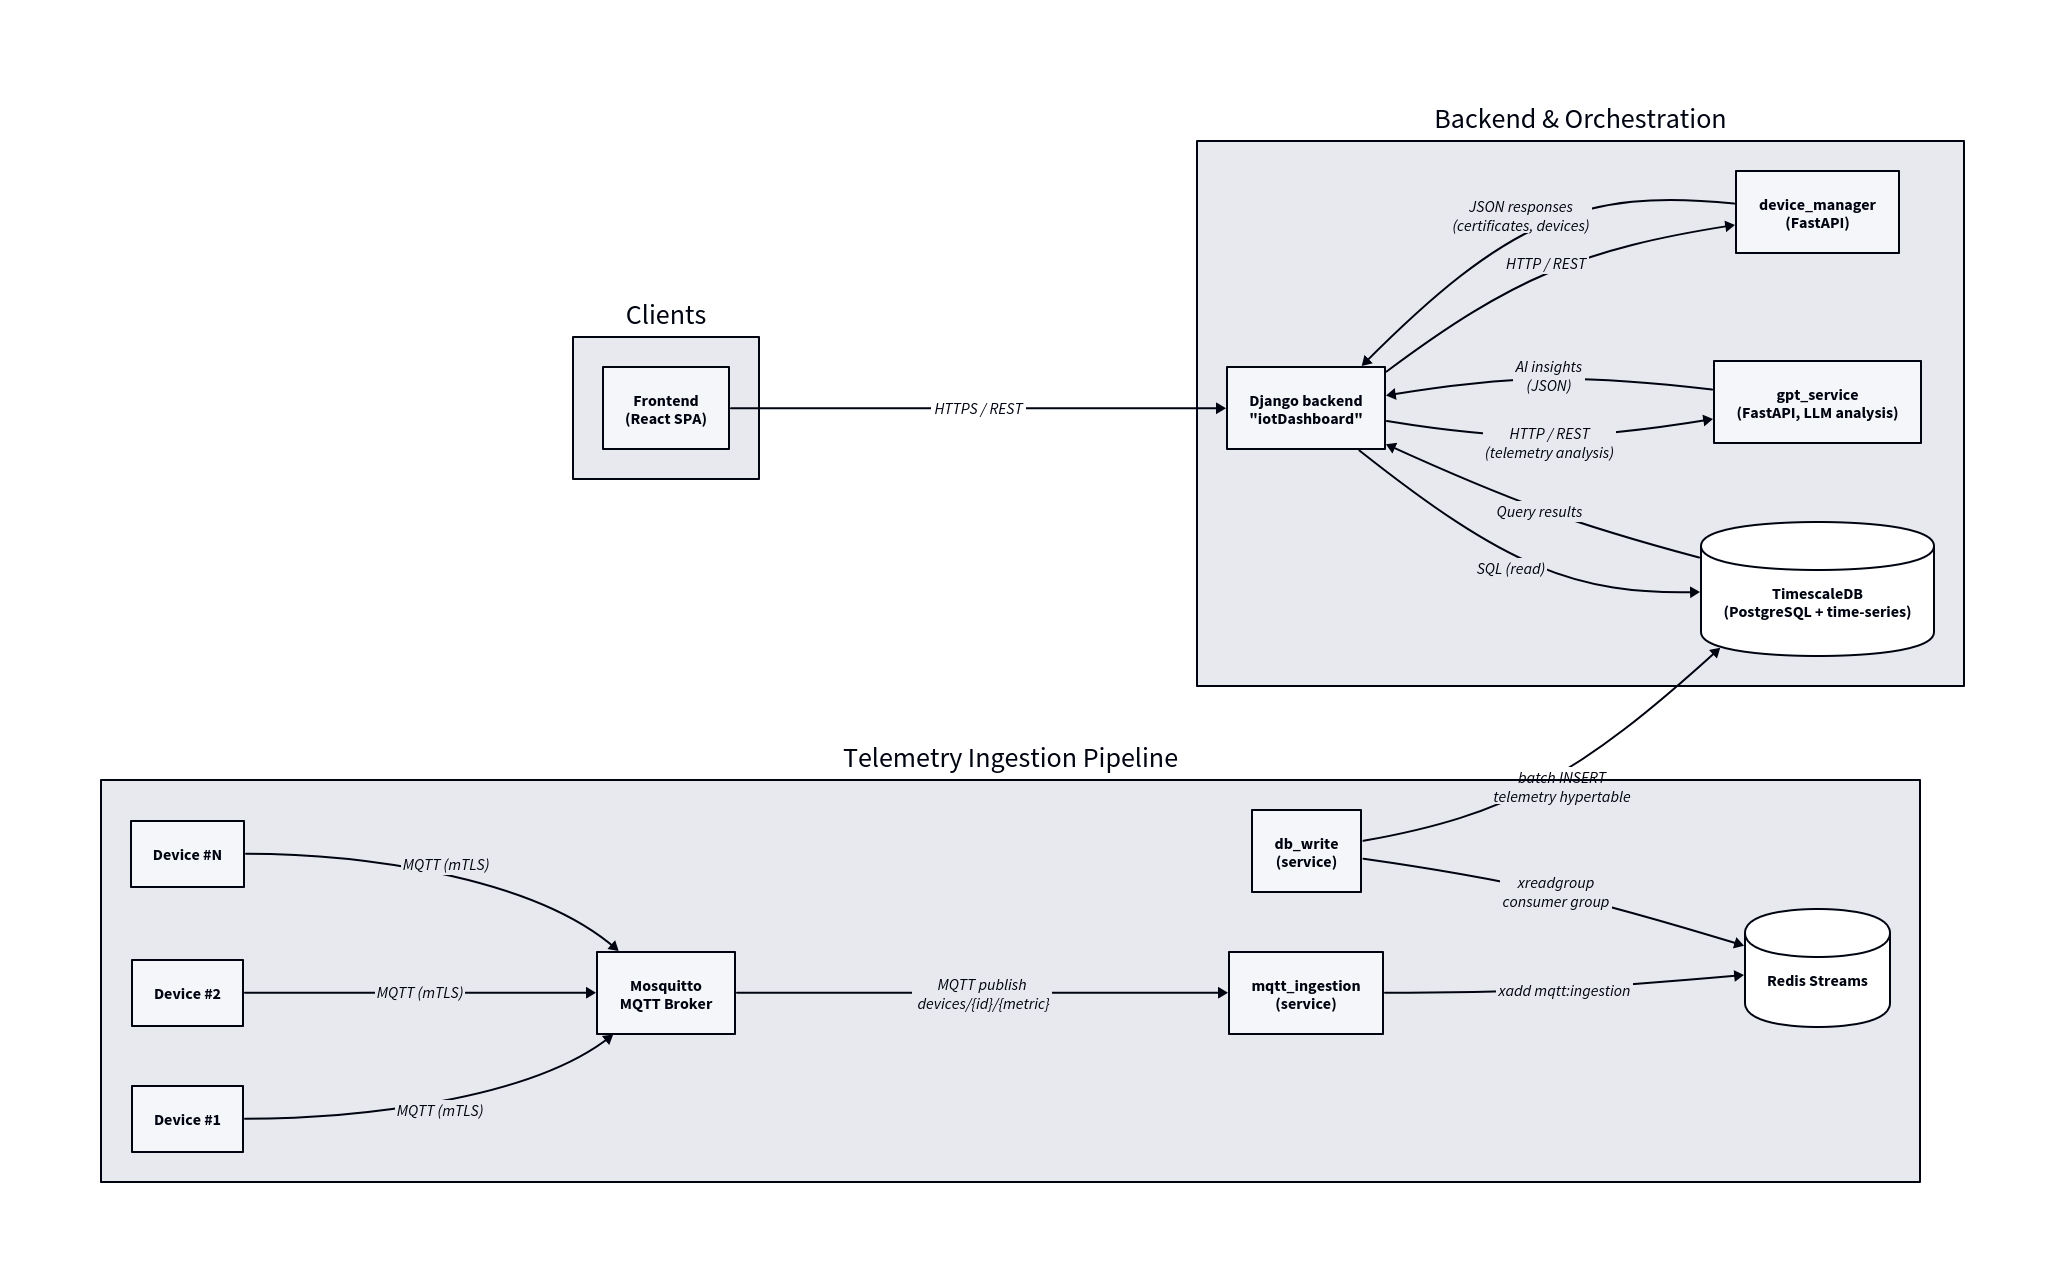
\includegraphics[width=\textwidth]{Miscellaneous/architecture.png}
    \caption{Архитектура на платформата за мониторинг на работна околина}
    \label{fig:system-architecture}
\end{figure}

\subsection{Проток на податоци}

Протокот на податоци во рамките на развиената платформа е дизајниран
така што овозможува сигурно, скалабилно и ефикасно движење на
информациите од крајните IoT уреди до веб интерфејсот. Процесот опфаќа
повеќе фази: регистрација на уред, безбедно поврзување преку mTLS,
испраќање и обработка на телеметриски податоци, нивно складирање во база
на податоци и конечно визуелизација преку frontend апликацијата.
Целокупниот тек е прикажан со дијаграм. (сл 3.2)

\subsubsection{Регистрација на уред}

Процесот започнува со регистрација на нов IoT уред во системот.
Корисникот иницира регистрација преку веб контролната табла имплементира
со React. При оваа постапка, frontend-от испраќа HTTP POST барање до
Django REST API кое содржи основни информации за уредот, како што се
име, локација и тип на уред.

Django го проследува ова барање кон интерниот \texttt{device\_manager}
микросервис, кој е задолжен за управување со уредите и нивните дигитални
сертификати. Device\_manager креира нов запис во табелата devices во
базата на податоци и иницира процес на генерирање на X.509 сертификат за
конкретниот уред. По успешното генерирање и потпишување на сертификатот
од страна на интерниот Certificate Authority (CA), приватниот клуч и
сертификатот му се враќаат на корисникот. Овие податоци понатаму се
имплементираат на самиот уред, со што тој станува подготвен за безбедно
поврзување на системот.

\subsubsection{Поврзување на уред преку mTLS}

По успешната регистрација, уредот иницира TCP конекција кон MQTT
\texttt{broker}-от преку порт-от 8883 кој е наменет за MQTT со SSL. При
воспоставување на конекцијата се извршува mTLS handshake постапка, при
што уредот го презентира својот X.509 сертификат пред \texttt{broker}-от, а
\texttt{broker}-от го презентира својот сертификат пред уредот.

\texttt{Mosquitto broker}-от врши верификација на сертификатот преку:

\begin{itemize}
\item
  Проверка на потписот од интерниот CA
\item
  Проверка на валидноста (датум на важност)
\item
  Проверка во Certificate Revocation List (CRL)
\end{itemize}

Доколку сите проверки се успешни, конекцијата се прифаќа и уредот добива
дозвола за publish. Во спротивно, доколку сертификатот е невалиден,
конекцијата автоматски се одбива.

\subsubsection{Испраќање и процесирање на телеметрија}

Откако уредот е успешно поврзан со MQTT \texttt{broker}-от, тој започнува со
публикување на телеметриски податоци на MQTT теми во облик
„devices/\{device\_id\}/\{metric\}`` каде што device\_id претставува
уникатен идентификатор на уредот, а metric го означува тимот на
измерениот параметар (на пр. Температура, влажност, CO2).

Сервисот \texttt{mqtt\_ingestion} е претплатен на сите релевантни теми и
функционира како централен приемник на сите MQTT пораки. По приемот на
секоја порака, податоците се парсираат и се запишуваат како нов запис во
Redis Stream-от \texttt{mqtt:ingestion}.

Сервисот \texttt{db\_write} функционира како consumer во рамките на \texttt{Redis}
\texttt{consumer group} и ги чита пораките од stream-от асинхроно. Податоците се
групираат и се запишуваат во \texttt{TimescaleDB} базата како нови записи во
\texttt{telemetry} \texttt{hypertable}. На овој начин се обезбедува висок проток на
податоци, buffering при оптоварување и at-least-once гаранција за
достава.

\subsubsection{Визуелизација и пристап до податоците}

Откако податоците се складирани во базата, тие стануваат достапни за
визуелизација преку веб-контролната табла. Frontend апликација направена
со React комуницира со Django REST API преку HTTP барања, при што API
слојот врши SQL барања за извлекување на податоците во зададените
временски интервали.

Добиените податоци се прикажуваат преку интерактивни графици, виџети и
табели, овозможувајќи им на корисниците да добијат увид во реално време
и историски во состојбата на работната околина и активностите.

\subsubsection{Интеграција на интелигентна анализа}

Покрај стандардната визуелизација, платформата овозможува интелигентна
анализа на податоците преку gpt\_service микросервисот. Овој сервис се
повикува директно со потребите податоци кои треба да ги обработи со
помош на AI модел и генерира текстуални анализи, препораки и детекција
на аномалии. Резултатите од AI анализата се прикажуваат во frontend
апликацијата како виџети што овозможува дополнителен слој на
интерпретација на постоечките податоци.

\subsection{Безбедносен модел на платформата}

Безбедноста е еден од клучните аспекти при дизајнот на оваа IoT
платформа, поради фактот што најголемиот дел од уредите се поставени во
небезбедни средини и комуницираат преку јавни мрежи. Класичната
автентикација, како што е споменато претходно, со корисничко име и
лозинка не е соодветна за вакви системи, бидејќи често претставува чест
извор на безбедности пропусти. Поради тоа, во рамките на оваа платформа
е имплементиран безбедносен модел базиран на mutual TLS (mTLS).

Кај mTLS, и клиентот (IoT уредот) и серверот (MQTT \texttt{broker}-от) меѓусебно
се автентицираат преку X.509 дигитални сертификати. На овој начин се
обезбедува двострана проверка на идентитетот, како и енкрипција и
интегритет на податоците при нивниот пренос. Секој уред поседува
уникатен сертификат, со што се овозможува прецизна идентификација и
контрола на пристапот до системот.

Во основата на овој модел се наоѓа интерен Certificate Authority (CA),
која ги потпишува сите сертификати во системот. Процесот на издавање на
сертификат се реализира преку \texttt{device\_manager} сервисот, кој при
регистрација на уред генерира сертификат и приватен клуч, ги складира
релевантните податоци во базата и му ги враќа на корисникот за
инсталација на уредот.

За управување со компромитирани или неактивни уреди се користи механизам
за повлекување на сертификати преку Certificate Revocation List (CRL).
При повлекување на сертификатот, тој се означува како невалиден во
системот, CRL листата се ажурира и MQTT \texttt{broker}-от автоматски го одбива
секој понатамошен обид за поврзување со тој сертификат.

Изборот на mTLS обезбедува високо ниво на безбедност, елиминација на
лозинки, силна криптографска идентификација на уредите и заштита од
напади како man-in-the-middle, што го прави овој пристап особено погоден
за IoT платформи.

\subsection{Дизајн на базата на податоци}

Складирањето на податоците во системот е дизајнирано така што овозможува
сигурно управување со уредите, дигиталните сертификати и телеметриските
мерења. Поради временската природа и големиот волумен на податоци,
базата на податоци е реализирана со \texttt{PostgreSQL} со \texttt{TimescaleDB}
екстензија.

\subsubsection{Табела \texttt{devices}}

Табелата \texttt{devices} ги содржи основните информации за секој регистриран
уред во системот во неа се складираат податоци како:

\begin{itemize}
\item
  Id - единствен идентификатор на уредот
\item
  name - име на уредот
\item
  Location - локација уредот
\item
  Created\_at - време на регистрација
\end{itemize}

Оваа табела претставува централна точка за поврзување на сите останати
податоци во системот

\subsubsection{Табела \texttt{device\_certificates}}

Табелата \texttt{device\_certificates} се користи за управување со X.509
сертификатите поврзани со уредите. Таа содржи:

\begin{itemize}
\item
  Id - сериски број на сертификатот
\item
  Device\_id - надворешен клуч кон табелата devices
\item
  Issued\_at - датум на издавање
\item
  Expires\_at -- датум на истекување
\item
  Revoked\_at - датум на повлекување (доколку постои)
\end{itemize}

Преку оваа табела се обезбедува информации за целиот животен циклус на
секој сертификат

\subsubsection{Табела \texttt{telemetry}}

Табелата \texttt{telemetry} претставува \texttt{TimescaleDB hypertable} и е
оптимизирана за складирање на временски серии од телеметриски податоци.
Таа содржи:

\begin{itemize}
\item
  Device\_id - идентификатор на уредот
\item
  Metric - тип на измерениот параметар
\item
  Value - измерена вредност
\item
  Timestamp - време на мерење
\end{itemize}

Податоците се автоматски партиционирани по време, што овозможува високо
ниво на ефикасност при внесување и пребарување на податоци. Примарниот
клуч е составен од (timestamp, device\_id, metric), што овозможува
оптимизирани прашалници при анализа на податоци по уред и временски
опсег.

\texttt{TimescaleDB} e избрана поради неколку технички предности како што се:

\begin{itemize}
\item
  Оптимизирана за работа со временски серии
\item
  Автоматска компресија
\item
  Континуирани агрегации за пресметка на просечни вредности
\item
  Скалабилност и компатибилност со \texttt{PostgreSQL}
\end{itemize}

Со ова се овозможува ефикасно, стабилно и долгорочно чување и користење
на телеметриските податоци од платформата. Целокупната структура на базата
на податоци е прикажана на ER дијаграмот (слика~\ref{fig:er-diagram}).

\begin{figure}[htbp]
    \centering
    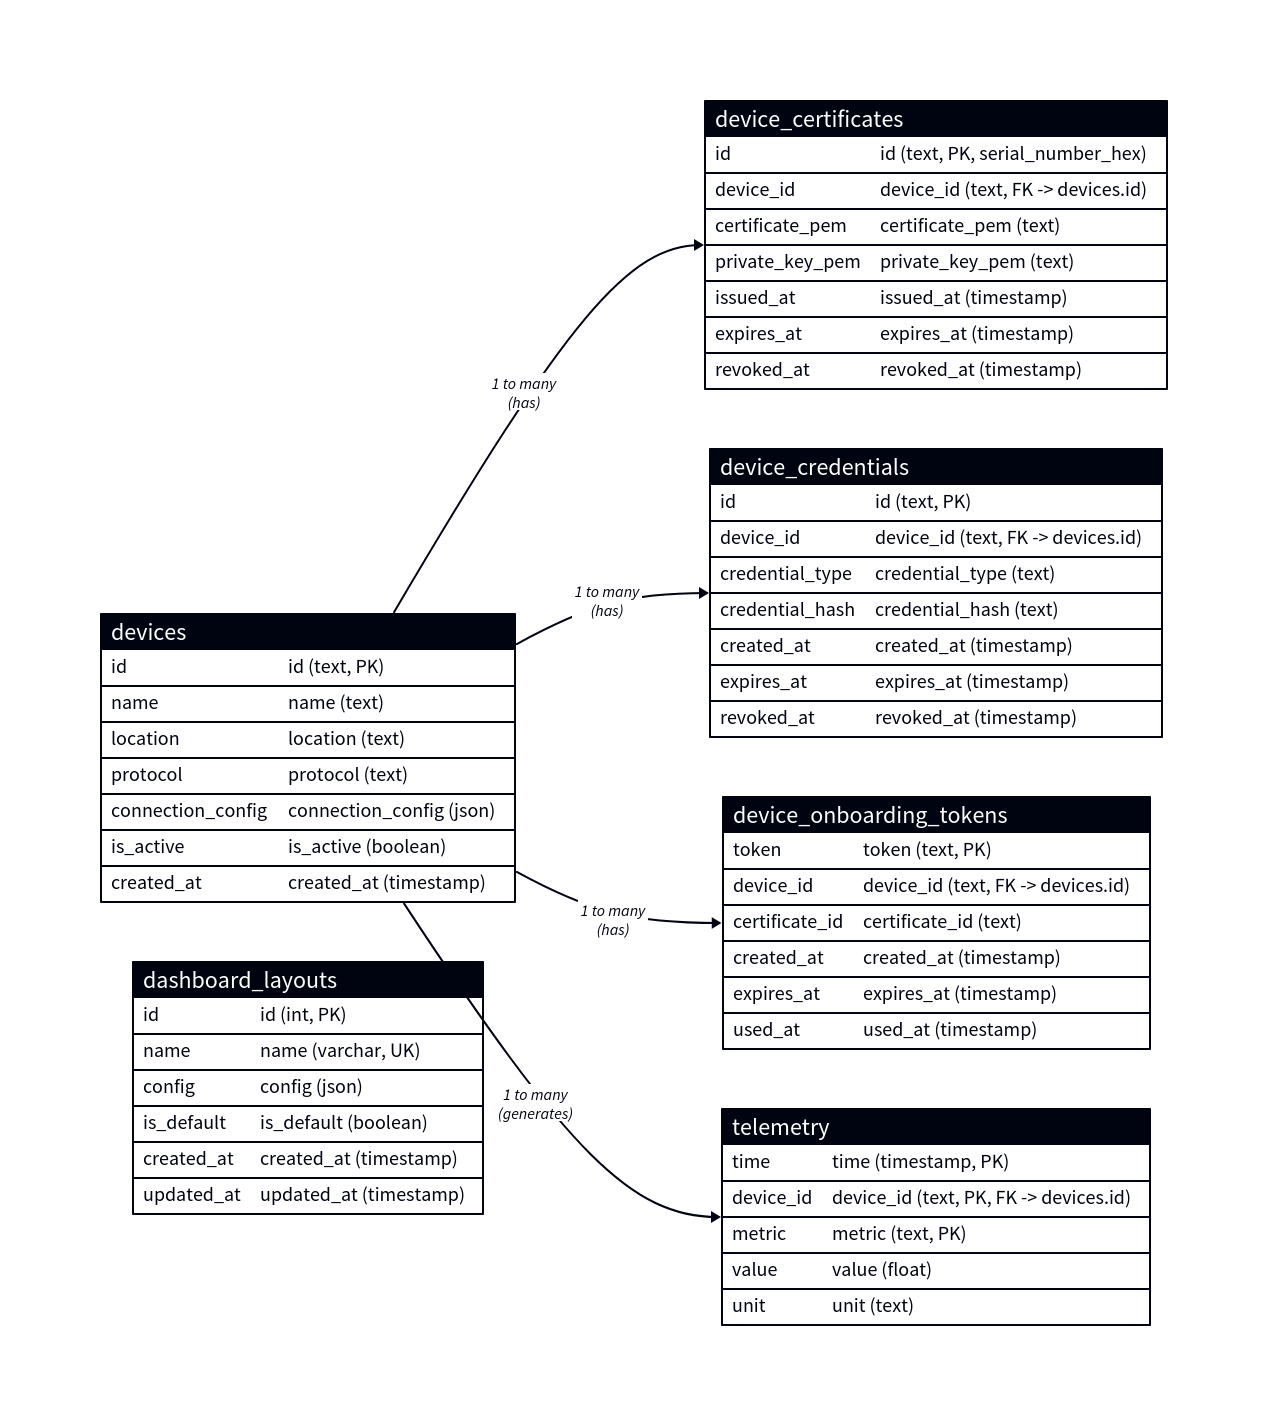
\includegraphics[width=\textwidth]{Miscellaneous/er_diagram.png}
    \caption{ER дијаграм на базата на податоци на платформата}
    \label{fig:er-diagram}
\end{figure}
